\begin{enumerate}[label=\thesection.\arabic*.,ref=\thesection.\theenumi]
\numberwithin{equation}{enumi}
\item Find the range of k such that given characteristic equation
\begin{align}
s(s^3+2s^2+s+1) +k(s^2+s+1) = 0
\label{eq:ee18btech11042_1}
\end{align}
is stable.

\solution
The General form of characteristic equation :
\begin{align}
1+G(s)H(s) = 0
\label{eq:ee18btech11042_2}    
\end{align}
\item  We draw nyquist plot for open loop transfer function, which is G(s)H(s). When system is marginally stable nyquist plot ((G(s)H(s))) passes through (-1,0),then 1+G(s)H(s) nyquist plot passes through (0,0). We will make real and imaginary part of characteristic equation to 0.So,that  we  get  k for system to be  marginally stable. For the system to be stable , the range of k becomes any value greater than k mimimum.
\begin{align}
Real part = \omega^4 - \omega^2(k+1) +k = 0
\label{eq:ee18btech11042_3}
\end{align}
\begin{align}
Imaginary part = -\omega^3 +\omega(w+1) = 0
\label{eq:ee18btech11042_4}
\end{align}
By equating real and imaginary to 0 .We get,
\begin{align}
 k = 0
\label{eq:ee18btech11042_5}
\end{align}
So,we got minimum value of k is 0 for system to be stable. Then the range of k is
\begin{align}
0<k<\infty
\label{eq:ee18btech11042_6}
\end{align}

\item For a nyquist plot,no.of clock wise encirclement's around the point(-1,0) for a open loop transfer function gives the total no. right hand side  zeros plus total no.of right hand side poles, which gives us a idea about stability of system.
\item   Nyquist plot for different values of k.

\begin{figure}[!h]
  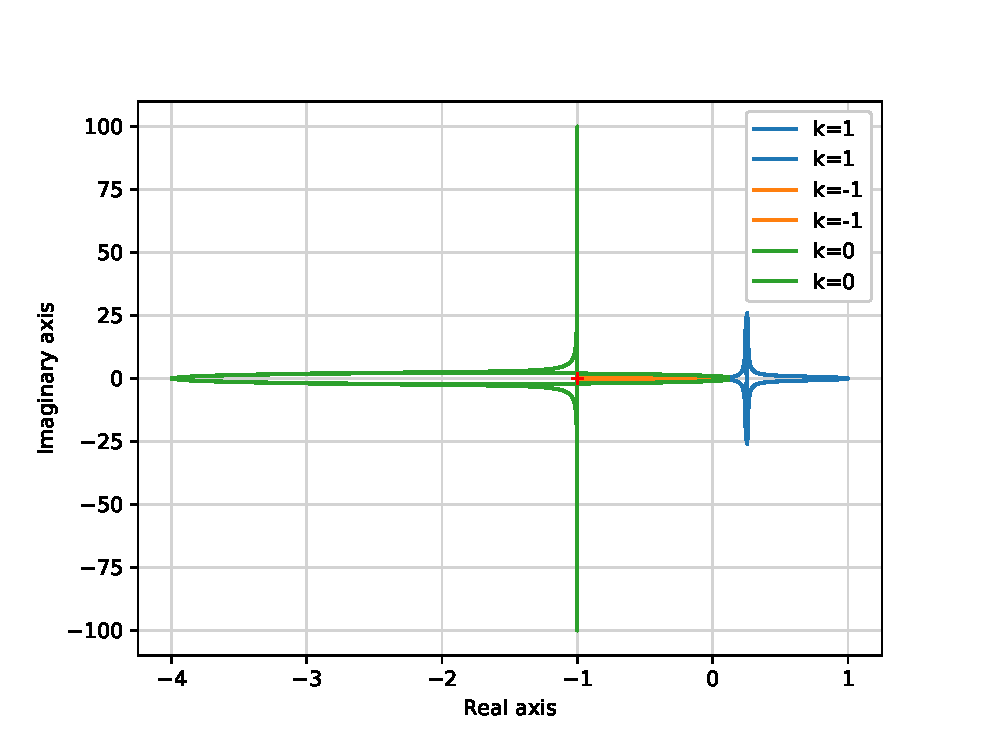
\includegraphics[width=\columnwidth]{.\figs\ee18btech11042_1.eps}
  \label{fig:ee18btech11042_1.eps}
\end{figure}
 In plot, we can see at k=0 ,the plot passes through (-1,0) and  at k = 1 no,of encirclements about (-1,0) is 0 which implies system is stable as no.of right  hand side zeros(positive values) are 0 and also verifies our above result of k range.
 

Code for Nyquist plot
\begin{lstlisting}
codes/ee18btech11042_1.py
\end{lstlisting}


\item Verify using Routh hurwitz criterion 
\newline
\solution
Routh -hurwitz criterion says system is marginally  when no.of sign changes is 0 in matrix and any row of matrix is completely 0. From this , we get minimum value of k for system to be stable

\begin{align}
s^4+2s^3+s^2(k+1)+s(k+1)+k = 0
\label{eq:ee18btech11042_7}
\end{align}
\mydet{s^4\\s^3\\s^2\\s^1\\s^0}
\mydet{1 & k+1 & k\\ 2 & k+1 & 0\\ \frac{k+1}{2} & k & 0\\ \frac{(k-1)^2}{2} & 0 & 0 \\ k & 0 & 0}
\item For the system to be stable,all values of that matrix should be greater than or equal to 0.So,minimum value of k is,


\begin{align}
k = 0
\label{eq:ee18btech11042_8}
\end{align}
The range of k system to be stable
\begin{align}
0<k<\infty
\label{eq:ee18btech11042_9}
\end{align}
\item Verify it using following routh -hurwitz code.
\begin{lstlisting}
codes/ee18btech11042_2.py
\end{lstlisting}
\end{enumerate}